% Date : 02/01/2023
% Version : 1
% Auteur : AEF
% Relu : 
% Relecteur : 

% ------------------------------------------------------------ %
% ----------------------  Fiche GAL03  ----------------------- %
% Thème : Signaux
% Classes : Toutes
% ------------------------------------------------------------ %

% ======================================================= % 
% ===================== Couleurs ======================== %
% ======================================================= % 

% -----------------------------------%
%  Définition de la couleur A de AEF
% Merci de préfixer vos couleur

% La commande \couleurNBouCouleur prend deux paramètres :
% #1 est la couleur NB ; #2 est la couleur "en couleur"

\def\AEFcouleurA{\couleurNBouCouleur{black}{blue}}
\def\AEFcouleurB{\couleurNBouCouleur{darkgray}{red}}
\def\AEFcouleurC{\couleurNBouCouleur{black}{orange}}



% ======================================================= % 
% ============== Gestion de la compilation ============== %
% ======================================================= % 
\ifdefined\mainIsLoaded\else
\RequirePackage{import}
\subimport{../../}{_preambule_CdE_PC}
\begin{document}
\fi
% ======================================================= % 
% ======================================================= % 






% ============================================================================ %
%                            FICHE D'ENTRAÎNEMENT                              %
% ============================================================================ %
% ======================= Métadonnées sur la fiche =========================== %
\titreFicheEntrainement		{Signaux}
\grandTheme					{Généralités}
\numeroFiche				{GAL03}
\uniqueID					{XZSYoCNJVcZ} % une chaîne de caractères (a-z, A-Z) aléatoire de 10 caractères.
\nombreColonnesReponses		{2} % 1, 2, 3, etc.
% ============================================================================ %

%%%%%%%%%%%%%%%%%%%%%%%%%%%%%%%%%%%%%%%%%%%%%%%%%%%%%%%%%%%%%%%%%%%%%%%%%%%%%%%%%%%%%%%%%%%%%%
\debutFicheEntrainement                                                                      %
%%%%%%%%%%%%%%%%%%%%%%%%%%%%%%%%%%%%%%%%%%%%%%%%%%%%%%%%%%%%%%%%%%%%%%%%%%%%%%%%%%%%%%%%%%%%%%




% --------------------------------------------------------------------- %
%                              Prérequis                                %
%                             (facultatif)                              %
% --------------------------------------------------------------------- %
% ================== Métadonnées sur le prérequis ===================== %
\avecPrerequis{Y} % Y ou N
% ===================================================================== %
\begin{prerequis}
	Fonctions trigonométriques. \\
	Signaux périodiques (fréquence, période, pulsation, longueur d'onde, phase).
\end{prerequis}
% --------------------------------------------------------------------- %




% •••••••••••••••••••••••••••••••••••••••••••••••••••••••••••••••••••••••••••• %
% •••••••••••••••••••••••••••••••••••••••••••••••••••••••••••••••••••••••••••• %
\sectionFicheEntrainement{Autour des fonctions trigonométriques}
% •••••••••••••••••••••••••••••••••••••••••••••••••••••••••••••••••••••••••••• %
% •••••••••••••••••••••••••••••••••••••••••••••••••••••••••••••••••••••••••••• %



% ********************************************************************* %
%                           ENTRAÎNEMENT                                % 
% ********************************************************************* %
% ================ Métadonnées sur l'entraînement ===================== %

\titreEntrainementFacultatif	{Cercle trigonométrique}
\hauteurLargeurCadreReponse		{8mm}{3cm}
\dureeResolutionFacultative		{1} % 1, 2, 3 ou 4
\typeEntrainement				{Newton} % Newton ou QCM ou AN ou vide (exercice "normal")
\basiqueEtTransversal			{Y}
\nombreColonnesQuestions		{2} % vide, 1, 2, 3, etc.
\avecPlusieursQuestions			{Y} % Y ou N
\initialisationEntrainement
% ===================================================================== %


% mmmmmmmmmmmmmmmmmmmmmmmmmmmmmmmmmmmmmmmmmmmmmmmmmmmmmmmmm %
% 		  Insertion d'une image en regard d'un texte
% mmmmmmmmmmmmmmmmmmmmmmmmmmmmmmmmmmmmmmmmmmmmmmmmmmmmmmmmm %
% --------------------------------------------------------- %
\pourcentageDeLaPartieAGauche   {0.6}
% --------------------------------------------------------- %
%                                                           %
% -------------------- Partie à gauche -------------------- %
%                                                           %
                                \initialisationPartieGauche % 
%                                                           %
%                                                           %
Sur le cercle trigonométrique ci-contre, $\cos(\alpha)$ se lit sur l'axe des abscisses et $\sin(\alpha)$ se lit sur l'axe des ordonnées. 


Exprimer les fonctions suivantes en fonction de $\cos(\alpha)$ et $\sin(\alpha)$.
% --------------------------------------------------------- %
%                                                           %
% -------------------- Partie à droite -------------------- %
%                                                           %
                                \initialisationPartieDroite %
%                                                           %
%                                                           %
\begin{center}
\subimport{_images/}{fiche_GAL03_cercle_trigo_CBD_v3.tex}
\end{center}
% --------------------------------------------------------- %
                               \finalisationDuPartageDePage %					
% --------------------------------------------------------- %


\medskip

% =============================================================================== %
\debutEntrainement
% =============================================================================== %

% ^^^^^^^^^^^^^^^^^^^^^^^^^^^^^^^^^^^^^^ %
%               Question                 %
% ^^^^^^^^^^^^^^^^^^^^^^^^^^^^^^^^^^^^^^ %

\begin{enonce}
$\sin(\alpha+\pi)$
\end{enonce}

\reponse{$-\sin(\alpha)$}

\begin{corrige}

% mmmmmmmmmmmmmmmmmmmmmmmmmmmmmmmmmmmmmmmmmmmmmmmmmmmmmmmmm %
% 		  Insertion d'une image en regard d'un texte
% mmmmmmmmmmmmmmmmmmmmmmmmmmmmmmmmmmmmmmmmmmmmmmmmmmmmmmmmm %
% --------------------------------------------------------- %
\pourcentageDeLaPartieAGauche   {0.65}
% --------------------------------------------------------- %
%                                                           %
% -------------------- Partie à gauche -------------------- %
%                                                           %
                                \initialisationPartieGauche % 
%                                                           %
%                                                           %
En utilisant le cercle trigonométrique, on voit directement que 
\[
\sin(\alpha+\pi)=-\sin(\alpha).
\]
 Remarquons qu'on peut également utiliser les formules trigonométriques : 
\[
\sin(\alpha+\pi)=\sin(\alpha)\cos(\pi)+\sin(\pi)\cos(\alpha)=-\sin(\alpha).
\]
% --------------------------------------------------------- %
%                                                           %
% -------------------- Partie à droite -------------------- %
%                                                           %
                                \initialisationPartieDroite %
%                                                           %
%                                                           %
\begin{center}
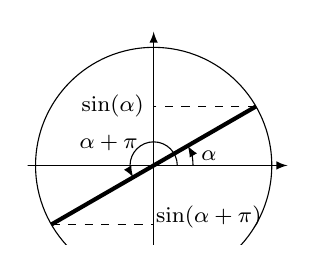
\begin{tikzpicture}
	\clip (-1.6,-1) rectangle (1.75,1.75);
	\draw(0,0) circle(1.5cm);
	\draw[->,>=latex](-1.7,0)--(1.7,0);
	\draw[->,>=latex](0,-1.7)--(0,1.7);
	\draw[line width=1.5pt](-1.3,-0.75) --(1.3,0.75);
	\draw[->,>=latex](0.5,0) arc (0: 30: 0.5cm)node[midway,right]{{\footnotesize $\textstyle{\alpha}$}};
	\draw[->,>=latex](0.3,0) arc (0: 210: 0.3cm)node[midway,left]{{\footnotesize $\textstyle{\alpha+\pi}$}};
	\draw[dashed](1.3,0.75)--(0,0.75)node[left]{{\footnotesize $\textstyle{\sin(\alpha)}$}};
	\draw[dashed](-1.3,-0.75)--(0,-0.75)node[xshift=0.7cm,yshift=0.1cm]{{\footnotesize $\sin(\alpha+\pi)$}};
\end{tikzpicture}
\end{center}
% --------------------------------------------------------- %
                               \finalisationDuPartageDePage %					
% --------------------------------------------------------- %

\end{corrige}

% ************************************** %

% ^^^^^^^^^^^^^^^^^^^^^^^^^^^^^^^^^^^^^^ %
%               Question                 %
% ^^^^^^^^^^^^^^^^^^^^^^^^^^^^^^^^^^^^^^ %

\begin{enonce}
$\cos(\alpha+\pi/2)$
\end{enonce}

\reponse{$-\sin(\alpha)$}

\begin{corrige}

% mmmmmmmmmmmmmmmmmmmmmmmmmmmmmmmmmmmmmmmmmmmmmmmmmmmmmmmmm %
% 		  Insertion d'une image en regard d'un texte
% mmmmmmmmmmmmmmmmmmmmmmmmmmmmmmmmmmmmmmmmmmmmmmmmmmmmmmmmm %
% --------------------------------------------------------- %
\pourcentageDeLaPartieAGauche   {0.65}
% --------------------------------------------------------- %
%                                                           %
% -------------------- Partie à gauche -------------------- %
%                                                           %
                                \initialisationPartieGauche % 
%                                                           %
%                                                           %
On a $\cos\left(\alpha+\dfrac{\pi}{2}\right)=-\sin(\alpha)$.

% --------------------------------------------------------- %
%                                                           %
% -------------------- Partie à droite -------------------- %
%                                                           %
                                \initialisationPartieDroite %
%                                                           %
%                                                           %
\begin{center}
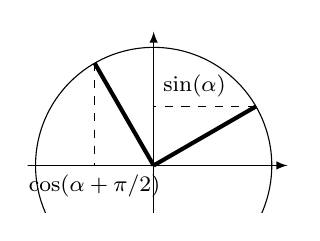
\begin{tikzpicture}
	\clip (-1.6,-0.6) rectangle (1.75,1.75);
	\draw(0,0) circle(1.5cm);
	\draw[->,>=latex](-1.7,0)--(1.7,0);
	\draw[->,>=latex](0,-1.7)--(0,1.7);
	\draw[line width=1.5pt](0,0) --(1.3,0.75);
	\draw[line width=1.5pt](0,0) --(-0.75,1.3);
	%\draw[->,>=latex](0.5,0) arc (0: 30: 0.5cm)node[midway,right]{$x$};
	%\draw[->,>=latex](0.5,0) arc (0: 120: 0.5cm)node[midway,above]{$x+\pi/2$};
	\draw[dashed](1.3,0.75)--(0,0.75)node[above right]{{\footnotesize $\sin(\alpha)$}};
	\draw[dashed](-0.75,1.3)--(-0.75,0)node[below]{{\footnotesize $\cos(\alpha+\pi/2)$}};
\end{tikzpicture}
\end{center}
% --------------------------------------------------------- %
                               \finalisationDuPartageDePage %					
% --------------------------------------------------------- %

\end{corrige}

% ************************************** %

% ^^^^^^^^^^^^^^^^^^^^^^^^^^^^^^^^^^^^^^ %
%               Question                 %
% ^^^^^^^^^^^^^^^^^^^^^^^^^^^^^^^^^^^^^^ %

\begin{enonce}
$\sin(\alpha+\pi/2)$
\end{enonce}

\reponse{$\cos(\alpha)$}

\begin{corrige}

% mmmmmmmmmmmmmmmmmmmmmmmmmmmmmmmmmmmmmmmmmmmmmmmmmmmmmmmmm %
% 		  Insertion d'une image en regard d'un texte
% mmmmmmmmmmmmmmmmmmmmmmmmmmmmmmmmmmmmmmmmmmmmmmmmmmmmmmmmm %
% --------------------------------------------------------- %
\pourcentageDeLaPartieAGauche   {0.65}
% --------------------------------------------------------- %
%                                                           %
% -------------------- Partie à gauche -------------------- %
%                                                           %
                                \initialisationPartieGauche % 
%                                                           %
%                                                           %
On a $\sin\left(\alpha+\dfrac{\pi}{2}\right)=\cos(\alpha)$.

% --------------------------------------------------------- %
%                                                           %
% -------------------- Partie à droite -------------------- %
%                                                           %
                                \initialisationPartieDroite %
%                                                           %
%                                                           %
\begin{center}
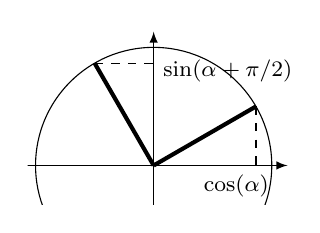
\begin{tikzpicture}
	\clip (-1.6,-0.5) rectangle (1.75,1.75);
	\draw(0,0) circle(1.5cm);
	\draw[->,>=latex](-1.7,0)--(1.7,0);
	\draw[->,>=latex](0,-1.7)--(0,1.7);
	\draw[line width=1.5pt](0,0) --(1.3,0.75);
	\draw[line width=1.5pt](0,0) --(-0.75,1.3);
	%\draw[->,>=latex](0.5,0) arc (0: 30: 0.5cm)node[midway,right]{$x$};
	%\draw[->,>=latex](0.5,0) arc (0: 120: 0.5cm)node[midway,above]{$x+\pi/2$};
	\draw[dashed](1.3,0.75)--(1.3,0)node[below,xshift=-0.25cm]{{\footnotesize $\cos(\alpha)$}};
	\draw[dashed](-0.75,1.3)--(0,1.3)node[right,yshift=-0.1cm]{{\footnotesize $\sin(\alpha+\pi/2)$}};
\end{tikzpicture}
\end{center}
% --------------------------------------------------------- %
                               \finalisationDuPartageDePage %					
% --------------------------------------------------------- %

\end{corrige}

% ************************************** %

% ^^^^^^^^^^^^^^^^^^^^^^^^^^^^^^^^^^^^^^ %
%               Question                 %
% ^^^^^^^^^^^^^^^^^^^^^^^^^^^^^^^^^^^^^^ %

\begin{enonce}
$\sin(\pi/2-\alpha)$
\end{enonce}

\reponse{$\cos(\alpha)$}

\begin{corrige}

% mmmmmmmmmmmmmmmmmmmmmmmmmmmmmmmmmmmmmmmmmmmmmmmmmmmmmmmmm %
% 		  Insertion d'une image en regard d'un texte
% mmmmmmmmmmmmmmmmmmmmmmmmmmmmmmmmmmmmmmmmmmmmmmmmmmmmmmmmm %
% --------------------------------------------------------- %
\pourcentageDeLaPartieAGauche   {0.65}
% --------------------------------------------------------- %
%                                                           %
% -------------------- Partie à gauche -------------------- %
%                                                           %
                                \initialisationPartieGauche % 
%                                                           %
%                                                           %
On a $\sin\left(\dfrac{\pi}{2}-\alpha\right)=\cos(\alpha)$.

% --------------------------------------------------------- %
%                                                           %
% -------------------- Partie à droite -------------------- %
%                                                           %
                                \initialisationPartieDroite %
%                                                           %
%                                                           %
\begin{center}
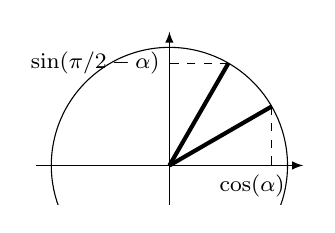
\begin{tikzpicture}
	\clip (-1.8,-0.5) rectangle (1.75,1.75);
	\draw(0,0) circle(1.5cm);
	\draw[->,>=latex](-1.7,0)--(1.7,0);
	\draw[->,>=latex](0,-1.7)--(0,1.7);
	\draw[line width=1.5pt](0,0) --(1.3,0.75);
	\draw[line width=1.5pt](0,0) --(0.75,1.3);
	%\draw[->,>=latex](0.5,0) arc (0: 30: 0.5cm)node[midway,right]{$x$};
	%\draw[->,>=latex](0.5,0) arc (0: 120: 0.5cm)node[midway,above]{$x+\pi/2$};
	\draw[dashed](1.3,0.75)--(1.3,0)node[below,xshift=-0.25cm]{{\footnotesize $\cos(\alpha)$}};
	\draw[dashed](0.75,1.3)--(0,1.3)node[left]{{\footnotesize $\sin(\pi/2-\alpha)$}};
\end{tikzpicture}
\end{center}
% --------------------------------------------------------- %
                               \finalisationDuPartageDePage %					
% --------------------------------------------------------- %

\end{corrige}

% ************************************** %

% =============================================================================== %
\finEntrainement
% =============================================================================== %









% ********************************************************************* %
%                           ENTRAÎNEMENT                                % 
% ********************************************************************* %
% ================ Métadonnées sur l'entraînement ===================== %

\titreEntrainementFacultatif	{Dérivée de signaux}
\hauteurLargeurCadreReponse		{8mm}{4cm}
\dureeResolutionFacultative		{1} % 1, 2, 3 ou 4
\typeEntrainement				{Newton} % Newton ou QCM ou AN ou vide (exercice "normal")
\basiqueEtTransversal			{Y}
\nombreColonnesQuestions		{2} % vide, 1, 2, 3, etc.
\avecPlusieursQuestions			{Y} % Y ou N
\initialisationEntrainement
% ===================================================================== %

Pour chaque signal ci-dessous, calculer sa dérivée par rapport à $t$.

% =============================================================================== %
\debutEntrainement
% =============================================================================== %


% ^^^^^^^^^^^^^^^^^^^^^^^^^^^^^^^^^^^^^^ %
%               Question                 %
% ^^^^^^^^^^^^^^^^^^^^^^^^^^^^^^^^^^^^^^ %

\begin{enonce}
$\sin(2t)$
\end{enonce}

\reponse{$2\cos(2t)$}

%\begin{corrige}
%\end{corrige}

% ************************************** %

% ^^^^^^^^^^^^^^^^^^^^^^^^^^^^^^^^^^^^^^ %
%               Question                 %
% ^^^^^^^^^^^^^^^^^^^^^^^^^^^^^^^^^^^^^^ %

\begin{enonce}
$\cos^2(t+4)$
\end{enonce}

\reponse{$-2\sin(t+4)\cos(t+4)=-\sin(2t+8)$}

%\begin{corrige}
%\end{corrige}

% ************************************** %


% ^^^^^^^^^^^^^^^^^^^^^^^^^^^^^^^^^^^^^^ %
%               Question                 %
% ^^^^^^^^^^^^^^^^^^^^^^^^^^^^^^^^^^^^^^ %

\begin{enonce}
$\cos(t)\times\sin(t)$
\end{enonce}

\reponse{$\cos^2(t)-\sin^2(t)=\cos(2t)$}

%\begin{corrige}
%\end{corrige}

% ************************************** %

% =============================================================================== %
\finEntrainement
% =============================================================================== %










% ********************************************************************* %
%                           ENTRAÎNEMENT                                % 
% ********************************************************************* %
% ================ Métadonnées sur l'entraînement ===================== %

\titreEntrainementFacultatif	{Transformer des sommes de signaux en produits}
\hauteurLargeurCadreReponse		{10mm}{9cm}
\dureeResolutionFacultative		{2} % 1, 2, 3 ou 4
\typeEntrainement				{Newton} % Newton ou QCM ou AN ou vide (exercice "normal")
\basiqueEtTransversal			{Y}
\nombreColonnesQuestions		{1} % vide, 1, 2, 3, etc.
\avecPlusieursQuestions			{Y} % Y ou N
\initialisationEntrainement
% ===================================================================== %



% =============================================================================== %
\debutEntrainement
% =============================================================================== %

On rappelle les formules trigonométriques : 
\begin{equation*}
\begin{aligned}
&\cos(a+b)=\cos(a)\cos(b)-\sin(a)\sin(b)\\
&\cos(a-b)=\cos(a)\cos(b)+\sin(a)\sin(b)\\
\end{aligned}
\hspace{1cm}
\begin{aligned}
&\sin(a+b)=\sin(a)\cos(b)+\cos(a)\sin(b)\\
&\sin(a-b)=\sin(a)\cos(b)-\cos(a)\sin(b).
\end{aligned}
\end{equation*}


Mettre les signaux suivants sous la forme $C\cos(\Omega t)\cos(\omega t)$ ou $C \sin(\Omega t)\sin(\omega t)$ (où les constantes $C$, $\Omega$ et $\omega$ s'exprimeront  en fonction de $A$, $\omega_1$ et $\omega_2$).


% ^^^^^^^^^^^^^^^^^^^^^^^^^^^^^^^^^^^^^^ %
%               Question                 %
% ^^^^^^^^^^^^^^^^^^^^^^^^^^^^^^^^^^^^^^ %

\begin{enonce}
$A\cos(\omega_1 t)+A\cos(\omega_2 t)$
\end{enonce}

\reponse{$2A\cos\left(\dfrac{\omega_1-\omega_2}{2}t\right)\cos\left(\dfrac{\omega_1+\omega_2}{2}t\right)$}

\begin{corrige}
On somme les formules trigonométriques : 
\begin{equation*}
\left\{\begin{aligned}
&\cos(a+b)=\cos(a)\cos(b)-\sin(a)\sin(b)\\
&\cos(a-b)=\cos(a)\cos(b)+\sin(a)\sin(b)\\
\end{aligned}\right.
\quad\text{ pour obtenir }\quad\cos(a+b)+\cos(a-b)=2\cos(a)\cos(b).
\end{equation*}

On a 
\begin{equation*}
\left\{\begin{aligned}
&a+b=\omega_1t\\
&a-b=\omega_2t\\
\end{aligned}\right.\ssi
\left\{\begin{aligned}
&a=\dfrac{\omega_1+\omega_2}{2}t\\
&b=\dfrac{\omega_1-\omega_2}{2}t.
\end{aligned}
\right.
\end{equation*}

On en déduit 
\begin{equation*}
A\cos(\omega_1 t)+A\cos(\omega_2 t)=2A\cos\left(\dfrac{\omega_1+\omega_2}{2}\, t\right)\cos\left(\dfrac{\omega_1-\omega_2}{2}\, t\right).
\end{equation*}

Ainsi, $C=2A$, $\Omega=\dfrac{\omega_1+\omega_2}{2}$ et $\omega=\dfrac{\omega_1-\omega_2}{2}$ conviennent.
\end{corrige}

% ************************************** %



% ^^^^^^^^^^^^^^^^^^^^^^^^^^^^^^^^^^^^^^ %
%               Question                 %
% ^^^^^^^^^^^^^^^^^^^^^^^^^^^^^^^^^^^^^^ %

\begin{enonce}
$A\cos(\omega_1 t)-A\cos(\omega_2 t)$
\end{enonce}

\reponse{$2A\sin\left(\dfrac{\omega_2-\omega_1}{2}t\right)\sin\left(\dfrac{\omega_1+\omega_2}{2}t\right)$}

\begin{corrige}
On somme les formules trigonométriques : 
\begin{equation*}
\left\{\begin{aligned}
&\cos(a+b)=\cos(a)\cos(b)-\sin(a)\sin(b)\\
&\cos(a-b)=\cos(a)\cos(b)+\sin(a)\sin(b)\\
\end{aligned}\right.
\quad\text{ pour obtenir }\quad\cos(a-b)-\cos(a+b)=2\sin(a)\sin(b).
\end{equation*}

On a 
\begin{equation*}
\left\{\begin{aligned}
&a-b=\omega_1t\\
&a+b=\omega_2t\\
\end{aligned}\right.\ssi
\left\{\begin{aligned}
&a=\dfrac{\omega_1+\omega_2}{2}t\\
&b=\dfrac{\omega_2-\omega_1}{2}t.
\end{aligned}
\right.
\end{equation*}

On en déduit  $A\cos(\omega_1 t)-A\cos(\omega_2 t)=2A\sin\left(\dfrac{\omega_2-\omega_1}{2}\, t\right)\sin\left(\dfrac{\omega_1+\omega_2}{2}\, t\right)$.
\end{corrige}

% ************************************** %


% =============================================================================== %
\finEntrainement
% =============================================================================== %






\newpage







% ********************************************************************* %
%                           ENTRAÎNEMENT                                % 
% ********************************************************************* %
% ================ Métadonnées sur l'entraînement ===================== %

\titreEntrainementFacultatif	{Formules d'addition}
\hauteurLargeurCadreReponse		{8mm}{10cm}
\dureeResolutionFacultative		{1} % 1, 2, 3 ou 4
\typeEntrainement				{Newton} % Newton ou QCM ou AN ou vide (exercice "normal")
\basiqueEtTransversal			{Y}
\nombreColonnesQuestions		{1} % vide, 1, 2, 3, etc.
\avecPlusieursQuestions			{N} % Y ou N
\initialisationEntrainement
% ===================================================================== %

Mettre le signal $A\sin(\omega t+\varphi)$ sous la forme $B\cos(\omega t)+C\sin(\omega t)$, où $B$ et $C$ dont des constantes à exprimer en fonction de $A$ et $\varphi$.

% =============================================================================== %
\debutEntrainement
% =============================================================================== %

% ^^^^^^^^^^^^^^^^^^^^^^^^^^^^^^^^^^^^^^ %
%               Question                 %
% ^^^^^^^^^^^^^^^^^^^^^^^^^^^^^^^^^^^^^^ %

\begin{enonce}
%Énoncé de la question.
\end{enonce}

\reponse{$A\sin(\varphi)\cos(\omega t)+A\cos(\varphi)\sin(\omega t)$}

\begin{corrige}
On utilise la formule trigonométrique : $\sin(a+b)=\sin(a)\cos(b)+\cos(a)\sin(b)$. 

On a $A\sin(\omega t+\varphi)=A\left[\sin(\omega t)\cos(\varphi)+\cos(\omega t)\sin(\varphi)\right]=A\sin(\varphi)\cos(\omega t)+A\cos(\varphi)\sin(\omega t)$. 

Ainsi, $B=A\sin(\varphi)$ et $C=A\cos(\varphi)$ conviennent.
\end{corrige}

% ************************************** %


% =============================================================================== %
\finEntrainement
% =============================================================================== %








% ********************************************************************* %
%                           ENTRAÎNEMENT                                % 
% ********************************************************************* %
% ================ Métadonnées sur l'entraînement ===================== %

\titreEntrainementFacultatif	{Représentations graphiques}
\hauteurLargeurCadreReponse		{8mm}{3cm}
\dureeResolutionFacultative		{1} % 1, 2, 3 ou 4
\typeEntrainement				{Newton} % Newton ou QCM ou AN ou vide (exercice "normal")
\basiqueEtTransversal			{Y}
\nombreColonnesQuestions		{2} % vide, 1, 2, 3, etc.
\avecPlusieursQuestions			{Y} % Y ou N
\initialisationEntrainement
% ===================================================================== %


\def\ratioGraphiqueX{1.15}
\def\ratioGraphiqueY{0.7}

\minusMedskip

\begin{center}
\subimport{_images/}{fiche_GAL03_graphique1_CBD_v3.tex}
\subimport{_images/}{fiche_GAL03_graphique2_CBD_v3.tex}
\bigskip

\subimport{_images/}{fiche_GAL03_graphique3_CBD_v3.tex}
\subimport{_images/}{fiche_GAL03_graphique4_CBD_v3.tex}
\end{center}
Pour les quatre graphiques ci-dessus, $\alpha$ est exprimé en radians. 

Associer chaque fonction à sa courbe représentative.


% =============================================================================== %
\debutEntrainement
% =============================================================================== %

% ^^^^^^^^^^^^^^^^^^^^^^^^^^^^^^^^^^^^^^ %
%               Question                 %
% ^^^^^^^^^^^^^^^^^^^^^^^^^^^^^^^^^^^^^^ %

\begin{enonce}
$\sin(\alpha)$
\end{enonce}

\reponse{Courbe 2}

\begin{corrige}
On a $\sin(0)=0$. La courbe 2 est la seule courbe passant par le point $(0,0)$ et est donc la seule courbe compatible. On vérifie aussi que la courbe 2 est comprise dans l'intervalle $[-1,1]$ et que sa période est égale à $2\pi$.
\end{corrige}

% ************************************** %


% ^^^^^^^^^^^^^^^^^^^^^^^^^^^^^^^^^^^^^^ %
%               Question                 %
% ^^^^^^^^^^^^^^^^^^^^^^^^^^^^^^^^^^^^^^ %

\begin{enonce}
$\cos(\alpha)$
\end{enonce}

\reponse{Courbe 4}

\begin{corrige}
On a $\cos(0)=1$, ce qui est cohérent avec les courbes 1, 3 et 4. Ce n'est donc pas suffisant pour déterminer quelle courbe correspond à la fonction cosinus. Mais on sait de plus que $\cos(x)\in[-1,1]$, ce qui correspond à la courbe 4. On vérifie également que la courbe 4 a une période égale à $2\pi$.
\end{corrige}

% ************************************** %


% ^^^^^^^^^^^^^^^^^^^^^^^^^^^^^^^^^^^^^^ %
%               Question                 %
% ^^^^^^^^^^^^^^^^^^^^^^^^^^^^^^^^^^^^^^ %

\begin{enonce}
$1+\sin(\alpha)$
\end{enonce}

\reponse{Courbe 3}

\begin{corrige}
On a $1+\sin(0)=1$ et $1+\sin(x)\in[0,2]$. Cela correspond à la courbe 3. On vérifie également que la courbe 3 a une période égale à $2\pi$.
\end{corrige}

% ************************************** %


% ^^^^^^^^^^^^^^^^^^^^^^^^^^^^^^^^^^^^^^ %
%               Question                 %
% ^^^^^^^^^^^^^^^^^^^^^^^^^^^^^^^^^^^^^^ %

\begin{enonce}
$\cos^2(\alpha)$
\end{enonce}

\reponse{Courbe 1}

\begin{corrige}
On a $\cos^2(0)=1$ et $\cos^2(x)\in[0,1]$. Cela correspond à la courbe 1. C'est aussi la seule courbe qui a une période égale à $\pi$.
\end{corrige}

% ************************************** %

% =============================================================================== %
\finEntrainement
% =============================================================================== %






% ********************************************************************* %
%                           ENTRAÎNEMENT                                % 
% ********************************************************************* %
% ================ Métadonnées sur l'entraînement ===================== %

\titreEntrainementFacultatif	{Formules trigonométriques}
\hauteurLargeurCadreReponse		{8mm}{1.5cm}
\dureeResolutionFacultative		{2} % 1, 2, 3 ou 4
\typeEntrainement				{QCM} % Newton ou QCM ou AN ou vide (exercice "normal")
\nombreColonnesQuestions		{1} % vide, 1, 2, 3, etc.
\avecPlusieursQuestions			{N} % Y ou N
\initialisationEntrainement
% ===================================================================== %

Le signal $\cos(\omega t)+\sin(\omega t)$ peut s'écrire sous la forme :

% =============================================================================== %
\debutEntrainement
% =============================================================================== %

% ^^^^^^^^^^^^^^^^^^^^^^^^^^^^^^^^^^^^^^ %
%               Question                 %
% ^^^^^^^^^^^^^^^^^^^^^^^^^^^^^^^^^^^^^^ %

\begin{enonce}
	\begin{listeQCM3Colonnes}
	\item $\cos^2(\omega t+\pi/4)$
	\item $2\cos(\omega t+\pi/4)$
	\item $\sqrt{2}\sin(\omega t+\pi/4)$\\
	\end{listeQCM3Colonnes}
	
\end{enonce}

\reponse{\reponseC}

\begin{corrige}
On peut mettre $A\sin(\omega t+\varphi)$ sous la forme $B\cos(\omega t)+C\sin(\omega t)$ avec $B=A\sin(\varphi)$ et $C=A\cos(\varphi)$. On a donc ici : 
\begin{equation*}
\left\{\begin{aligned}
&A\sin(\varphi)=1\\
&A\cos(\varphi)=1\\
\end{aligned}\right.
\end{equation*}

En faisant le rapport des deux équations, on obtient $\dfrac{\sin(\varphi)}{\cos(\varphi)}=\tan(\varphi)=1$, ce qui correspond à $\varphi=\dfrac{\pi}{4}$. 

On utilise alors la première équation : $A\sin\left(\dfrac{\pi}{4}\right)=\dfrac{A}{\sqrt{2}}=1$. Donc, $A=\sqrt{2}$. 

Finalement, $\cos(\omega t)+\sin(\omega t)=\sqrt{2}\sin(\omega t+\pi/4)$ ce qui correspond à la réponse \reponseC . 
\end{corrige}

% ************************************** %


% =============================================================================== %
\finEntrainement
% =============================================================================== %






\newpage



% •••••••••••••••••••••••••••••••••••••••••••••••••••••••••••••••••••••••••••• %
% •••••••••••••••••••••••••••••••••••••••••••••••••••••••••••••••••••••••••••• %
\sectionFicheEntrainement{\'Etude graphique}
% •••••••••••••••••••••••••••••••••••••••••••••••••••••••••••••••••••••••••••• %
% •••••••••••••••••••••••••••••••••••••••••••••••••••••••••••••••••••••••••••• %



% ********************************************************************* %
%                           ENTRAÎNEMENT                                % 
% ********************************************************************* %
% ================ Métadonnées sur l'entraînement ===================== %

\titreEntrainementFacultatif	{Paramètres d'un signal sinusoïdal}
\hauteurLargeurCadreReponse		{8mm}{2.5cm}
\dureeResolutionFacultative		{1} % 1, 2, 3 ou 4
\typeEntrainement				{Newton} % Newton ou QCM ou AN ou vide (exercice "normal")
\nombreColonnesQuestions		{2} % vide, 1, 2, 3, etc.
\avecPlusieursQuestions			{Y} % Y ou N
\initialisationEntrainement
% ===================================================================== %



En travaux pratiques, vous faites l'acquisition d'une tension sinusoïdale $u(t)=U_0\cos\left(\dfrac{2\pi}{T}t+\varphi\right)$ et obtenez l'oscillogramme ci-dessous. 

\def\ratioGraphiqueX{1.1}
\def\ratioGraphiqueY{0.7}

\begin{center}
\subimport{_images/}{fiche_GAL03_graphe_sinus_CBD_v4.tex}
\end{center}

Par lecture graphique ou par le calcul, déterminer :

% =============================================================================== %
\debutEntrainement
% =============================================================================== %


% ^^^^^^^^^^^^^^^^^^^^^^^^^^^^^^^^^^^^^^ %
%               Question                 %
% ^^^^^^^^^^^^^^^^^^^^^^^^^^^^^^^^^^^^^^ %

\begin{enonce}
l'amplitude $U_0$
\end{enonce}

\reponse{$\SI{1,5}{V}$}

%\begin{corrige}
%\end{corrige}

% ************************************** %

% ^^^^^^^^^^^^^^^^^^^^^^^^^^^^^^^^^^^^^^ %
%               Question                 %
% ^^^^^^^^^^^^^^^^^^^^^^^^^^^^^^^^^^^^^^ %

\begin{enonce}
la phase à l'origine $\varphi$
\end{enonce}

\reponse{$\frac{\pi}{2}\;\si{rad}$}

\begin{corrige}
On lit graphiquement $u(0)=0=U_0\cos(\varphi)$. Donc, $\cos(\varphi)=0$. Donc, $\varphi=\dfrac{\pi}{2}$.
\end{corrige}

% ************************************** %

% ^^^^^^^^^^^^^^^^^^^^^^^^^^^^^^^^^^^^^^ %
%               Question                 %
% ^^^^^^^^^^^^^^^^^^^^^^^^^^^^^^^^^^^^^^ %

\begin{enonce}
la période $T$
\end{enonce}

\reponse{$\SI{2}{s}$}

%\begin{corrige}
%\end{corrige}

% ************************************** %

% ^^^^^^^^^^^^^^^^^^^^^^^^^^^^^^^^^^^^^^ %
%               Question                 %
% ^^^^^^^^^^^^^^^^^^^^^^^^^^^^^^^^^^^^^^ %

\begin{enonce}
la fréquence $f$
\end{enonce}

\reponse{$\SI{0,5}{Hz}$}

\begin{corrige}
On a mesuré à la question précédente $T=\SI{2}{s}$. D'où $f=\dfrac{1}{T}=\SI{0,5}{Hz}$.
\end{corrige}

% ************************************** %

% ^^^^^^^^^^^^^^^^^^^^^^^^^^^^^^^^^^^^^^ %
%               Question                 %
% ^^^^^^^^^^^^^^^^^^^^^^^^^^^^^^^^^^^^^^ %

\begin{enonce}
la pulsation $\omega$.
\end{enonce}

\reponse{$\pi\;\si{rad.s^{-1}}$}

\begin{corrige}
On a déterminé $f=\SI{0,5}{Hz}$ à la question précédente, d'où $\omega=2\pi f=\pi\;\si{rad.s^{-1}}$.
\end{corrige}

% ************************************** %


% =============================================================================== %
\finEntrainement
% =============================================================================== %





% ********************************************************************* %
%                           ENTRAÎNEMENT                                % 
% ********************************************************************* %
% ================ Métadonnées sur l'entraînement ===================== %

\titreEntrainementFacultatif	{Différence de phase}
\hauteurLargeurCadreReponse		{8mm}{5cm}
\dureeResolutionFacultative		{1} % 1, 2, 3 ou 4
\typeEntrainement				{Newton} % Newton ou QCM ou AN ou vide (exercice "normal")
\nombreColonnesQuestions		{1} % vide, 1, 2, 3, etc.
\avecPlusieursQuestions			{Y} % Y ou N
\initialisationEntrainement
% ===================================================================== %

La figure ci-dessous donne les représentations graphiques de deux signaux : le signal $u_1(t)=U_0\cos(\omega t)$ et le signal $u_2(t)=U_0\cos(\omega t+\varphi)$, où on a $\omega=\frac{2\pi}{3}\; \si{rad.s^{-1}}$.

\def\ratioGraphiqueX{1.1}
\def\ratioGraphiqueY{0.7}

\begin{center}
\subimport{_images/}{fiche_GAL03_phase_CBD_v3.tex}
\end{center}

% =============================================================================== %
\debutEntrainement
% =============================================================================== %


% ^^^^^^^^^^^^^^^^^^^^^^^^^^^^^^^^^^^^^^ %
%               Question                 %
% ^^^^^^^^^^^^^^^^^^^^^^^^^^^^^^^^^^^^^^ %

\begin{enonce}
Le signal $u_2(t)$ est-il en avance ou en retard sur $u_1(t)$ ?
\end{enonce}

\reponse{En retard}

\begin{corrige}
Le signal $u_1(t)$ atteint son premier maximum avant $u_2(t)$. Le signal $u_2(t)$ est donc en retard sur $u_1(t)$.
\end{corrige}

% ************************************** %


% ^^^^^^^^^^^^^^^^^^^^^^^^^^^^^^^^^^^^^^ %
%               Question                 %
% ^^^^^^^^^^^^^^^^^^^^^^^^^^^^^^^^^^^^^^ %

\begin{enonce}
En déduire le signe de $\varphi$.
\end{enonce}

\reponse{$\varphi<0$}

%\begin{corrige}
%\end{corrige}

% ************************************** %


% ^^^^^^^^^^^^^^^^^^^^^^^^^^^^^^^^^^^^^^ %
%               Question                 %
% ^^^^^^^^^^^^^^^^^^^^^^^^^^^^^^^^^^^^^^ %

\begin{enonce}
Déterminer graphiquement $\varphi$.
\end{enonce}

\reponse{$-\frac{2\pi}{3}\;\si{rad}$}

\begin{corrige}
On lit graphiquement le retard $\tau=\SI{-1}{s}$ de $u_2(t)$ sur $u_1(t)$. On en déduit $\varphi=\omega \tau=-\frac{2\pi}{3}\;\si{rad}$.
\end{corrige}

% ************************************** %


% =============================================================================== %
\finEntrainement
% =============================================================================== %




% ********************************************************************* %
%                           ENTRAÎNEMENT                                % 
% ********************************************************************* %
% ================ Métadonnées sur l'entraînement ===================== %
\pointInterrogation				{Y}
\titreEntrainementFacultatif	{Qui est qui}
\hauteurLargeurCadreReponse		{6mm}{1.5cm}
\dureeResolutionFacultative		{2} % 1, 2, 3 ou 4
\typeEntrainement				{Newton} % Newton ou QCM ou AN ou vide (exercice "normal")
\nombreColonnesQuestions		{3} % vide, 1, 2, 3, etc.
\avecPlusieursQuestions			{Y} % Y ou N
\initialisationEntrainement
% ===================================================================== %

En travaux pratiques, vous faites l'acquisition de trois signaux périodiques : $u_1(t)$, $u_2(t)$ et $u_3(t)$. 

Malheureusement, vous ne vous souvenez pas quelle voie d'acquisition vous avez utilisée pour chaque signal !

Vous savez que la tension $u_1(t)$ a pour période $\SI{300}{\micro s}$, que la tension $u_2(t)$ a pour fréquence $\SI{8,0}{\kilo Hz}$ et que la tension $u_3(t)$ a pour pulsation $\SI{1e4}{rad.s^{-1}}$.

\def\ratioGraphiqueX{1.12}
\def\ratioGraphiqueY{0.8}

\minusMedskip

\begin{center}
\subimport{_images/}{fiche_GAL03_qui_est_qui_CBD_v3.tex}
\end{center}

Attribuer chacun des graphes au signal qui lui correspond.

% =============================================================================== %
\debutEntrainement
% =============================================================================== %

% ^^^^^^^^^^^^^^^^^^^^^^^^^^^^^^^^^^^^^^ %
%               Question                 %
% ^^^^^^^^^^^^^^^^^^^^^^^^^^^^^^^^^^^^^^ %

\begin{enonce}
Voie A 
\end{enonce}

\reponse{$u_3(t)$}


% ************************************** %
% ^^^^^^^^^^^^^^^^^^^^^^^^^^^^^^^^^^^^^^ %
%               Question                 %
% ^^^^^^^^^^^^^^^^^^^^^^^^^^^^^^^^^^^^^^ %

\begin{enonce}
Voie B 
\end{enonce}

\reponse{$u_1(t)$}


% ************************************** %
% ^^^^^^^^^^^^^^^^^^^^^^^^^^^^^^^^^^^^^^ %
%               Question                 %
% ^^^^^^^^^^^^^^^^^^^^^^^^^^^^^^^^^^^^^^ %

\begin{enonce}
Voie C 
\end{enonce}

\reponse{$u_2(t)$}

\begin{corrige}
Le signal $u_1(t)$ a pour période $T_1=\SI{300}{\micro s}$. Le signal $u_2(t)$ a pour période $T_2=\dfrac{1}{f_2}=\SI{125}{\micro s}$. Enfin, le signal $u_3(t)$ a pour période $T_3=\dfrac{2\pi}{\omega_3}=\SI{628}{\micro s}$. On classe donc les trois signaux par ordre croissant de période : $T_2<T_1<T_3$ puis par identification : $u_3(t)\longleftrightarrow$ Voie A ; $u_1(t)\longleftrightarrow$ Voie B ; $u_2(t)\longleftrightarrow$ Voie C.
\end{corrige}

% ************************************** %

% =============================================================================== %
\finEntrainement
% =============================================================================== %



\medskip


% •••••••••••••••••••••••••••••••••••••••••••••••••••••••••••••••••••••••••••• %
% •••••••••••••••••••••••••••••••••••••••••••••••••••••••••••••••••••••••••••• %
\sectionFicheEntrainement{Valeur moyenne et valeur efficace}
% •••••••••••••••••••••••••••••••••••••••••••••••••••••••••••••••••••••••••••• %
% •••••••••••••••••••••••••••••••••••••••••••••••••••••••••••••••••••••••••••• %

\medskip

La valeur moyenne $U_{\text{moy}}$  et la valeur efficace $U_{\textrm{eff}}$ d'un signal $u(t)$ périodique de période $T$ sont définies par les formules : 
\[
U_{\text{moy}}=\dfrac{1}{T}\int_0^T \!\!u(t)\d{}t
\qquad\text{et}\qquad
U_{\textrm{eff}}=\sqrt{\dfrac{1}{T}\int_0^T \!\!u(t)^2\d{}t}.
\]
\minusMedskip

% ********************************************************************* %
%                           ENTRAÎNEMENT                                % 
% ********************************************************************* %
% ================ Métadonnées sur l'entraînement ===================== %

\titreEntrainementFacultatif	{Signal sinusoïdal}
\hauteurLargeurCadreReponse		{8mm}{5cm}
\dureeResolutionFacultative		{3} % 1, 2, 3 ou 4
\typeEntrainement				{Newton} % Newton ou QCM ou AN ou vide (exercice "normal")
\basiqueEtTransversal			{Y}
\nombreColonnesQuestions		{1} % vide, 1, 2, 3, etc.
\avecPlusieursQuestions			{Y} % Y ou N
\initialisationEntrainement
% ===================================================================== %

On considère le signal sinusoïdal $u(t)=U_0\cos\left(\dfrac{2\pi}{T}t\right)$.

% =============================================================================== %
\debutEntrainement
% =============================================================================== %

% ^^^^^^^^^^^^^^^^^^^^^^^^^^^^^^^^^^^^^^ %
%               Question                 %
% ^^^^^^^^^^^^^^^^^^^^^^^^^^^^^^^^^^^^^^ %

\begin{enonce}
Calculer la valeur moyenne de $u(t)$
\end{enonce}

\reponse{$0$}

\begin{corrige}
Par définition, on a $U_{\text{moy}}=\dfrac{1}{T}\int_0^T\!\!u(t)\d{}t$. On calcule donc : 
\begin{equation*}
U_{\text{moy}}=\dfrac{1}{T}\int_0^TU_0\cos\left(\dfrac{2\pi}{T}t\right)\d{}t=\dfrac{U_0}{T}\times\dfrac{T}{2\pi}\left[\sin\left(\dfrac{2\pi}{T}t\right)\right]_0^T=\dfrac{U_0}{2\pi}\left(0-0\right)=0.
\end{equation*}
\end{corrige}

% ************************************** %

% ^^^^^^^^^^^^^^^^^^^^^^^^^^^^^^^^^^^^^^ %
%               Question                 %
% ^^^^^^^^^^^^^^^^^^^^^^^^^^^^^^^^^^^^^^ %

\begin{enonce}
Calculer la valeur efficace de $u(t)$
\end{enonce}

\reponse{$\frac{U_0}{\sqrt{2}}$}

% ************************************** %

\begin{corrige}
Par définition, on a $U_{\textrm{eff}}=\sqrt{\dfrac{1}{T}\int_0^T \!\!u(t)^2\d{}t}$.
On calcule donc : ${U_{\textrm{eff}}}^2=\dfrac{1}{T}\int_0^T\!\!U_0^2\cos^2\left(\dfrac{2\pi}{T}t\right)\d{}t$.

Pour calculer cette intégrale, il faut linéariser le cosinus au carré. Pour cela, on peut utiliser les formules trigonométriques : 
\begin{equation*}
\cos(2x)=\cos^2(x)-\sin^2(x)=2\cos^2(x)-1\qquad\text{donc}\qquad\cos^2(x)=\dfrac{1+\cos(2x)}{2}.
\end{equation*}
D'où,
\[
{U_\textrm{eff}}^2=\dfrac{U_0^2}{T}\int_0^T\!\!\bigg(\dfrac{1}{2}+\dfrac{\cos\left(\dfrac{2\pi}{T}t\right)}{2}\bigg)\d{}t=
%\dfrac{U_0^2}{2}\left(\dfrac{1}{T}\int_0^T\!\!\!\d{}t+U_{\text{moy}}\right)=\dfrac{U_0^2}{2}.
\dfrac{U_0^2}{2}\left(\dfrac{1}{T}\int_0^T\!\!\!\d{}t\right) + \frac{U_0}{2}U_{\text{moy}}=\dfrac{U_0^2}{2}.
\]
Ainsi, $U_\textrm{eff}=\dfrac{U_0}{\sqrt{2}}$.
\end{corrige}

% =============================================================================== %
\finEntrainement
% =============================================================================== %


\newpage





% ********************************************************************* %
%                           ENTRAÎNEMENT                                % 
% ********************************************************************* %
% ================ Métadonnées sur l'entraînement ===================== %

\titreEntrainementFacultatif	{Un signal carré}
\hauteurLargeurCadreReponse		{8mm}{2cm}
\dureeResolutionFacultative		{2} % 1, 2, 3 ou 4
\typeEntrainement				{Newton} % Newton ou QCM ou AN ou vide (exercice "normal")
\basiqueEtTransversal			{Y}
\nombreColonnesQuestions		{2} % vide, 1, 2, 3, etc.
\avecPlusieursQuestions			{Y} % Y ou N
\initialisationEntrainement
% ===================================================================== %


On considère le signal périodique carré dissymétrique $u(t)$ représenté ci-dessous.
                                                 %
\def\ratioGraphiqueX{1.12}
\def\ratioGraphiqueY{0.8}
\begin{center}
\subimport{_images/}{fiche_GAL03_carre_CBD_v3.tex}
\end{center}

\minusMedskip
Calculer : 
\minusMedskip

% =============================================================================== %
\debutEntrainement
% =============================================================================== %

% ^^^^^^^^^^^^^^^^^^^^^^^^^^^^^^^^^^^^^^ %
%               Question                 %
% ^^^^^^^^^^^^^^^^^^^^^^^^^^^^^^^^^^^^^^ %

\begin{enonce}
la valeur moyenne de $u(t)$
\end{enonce}

\reponse{$\SI{1,5}{V}$}

\begin{corrige}
On lit graphiquement que la période est $T=\SI{4}{s}$ et que, sur une période, le signal prend les valeurs :
\begin{equation*}
u(t) =
\left|
\begin{aligned}
&\SI{3}{V}\textrm{ si }\SI{0}{s}<t\leq \SI{1}{s}\\
&\SI{1}{V}\textrm{ si }\SI{1}{s}<t\leq \SI{4}{s}.
\end{aligned}
\right.
\end{equation*}

On calcule donc : 
\begin{equation*}
U_{\text{moy}}=\dfrac{1}{4}\bigg(\int_0^1 \!\! 3\d{}t+\int_1^4 \!\! 1\d{}t\bigg)=\dfrac{1}{4}\left(3+3\right)=\dfrac{6}{4}=\SI{1,5}{V}.
\end{equation*}
\end{corrige}

% ************************************** %


% ^^^^^^^^^^^^^^^^^^^^^^^^^^^^^^^^^^^^^^ %
%               Question                 %
% ^^^^^^^^^^^^^^^^^^^^^^^^^^^^^^^^^^^^^^ %

\begin{enonce}
la valeur efficace de $u(t)$
\end{enonce}

\reponse{$\sqrt{3}\;\si{V}$}

\begin{corrige}
On a toujours $T=\SI{4}{s}$ et 
\begin{equation*}
u(t)=
\left|
\begin{aligned}
&\SI{3}{V} \textrm{ si }\SI{0}{s}<t\leq \SI{1}{s}\\
&\SI{1}{V} \textrm{ si }\SI{1}{s}<t\leq \SI{4}{s}.
\end{aligned}
\right.
\end{equation*}

On calcule donc : 

\begin{equation*}
{U_{\text{eff}}}^2=\dfrac{1}{4}\bigg(\int_0^1\!\!9\d{}t+\int_1^4\!\!1\d{}t\bigg)=\dfrac{1}{4}\left(9+3\right)=\dfrac{12}{4}=\SI{3}{V^2}.
\end{equation*}
Donc, $U_{\text{eff}}=\sqrt{3}\;\si{V}$.
\end{corrige}

% ************************************** %


% =============================================================================== %
\finEntrainement
% =============================================================================== %






% ********************************************************************* %
%                           ENTRAÎNEMENT                                % 
% ********************************************************************* %
% ================ Métadonnées sur l'entraînement ===================== %

\titreEntrainementFacultatif	{Un signal carré, sans son dessin}
\hauteurLargeurCadreReponse		{8mm}{2cm}
\dureeResolutionFacultative		{1} % 1, 2, 3 ou 4
\typeEntrainement				{Newton} % Newton ou QCM ou AN ou vide (exercice "normal")
\basiqueEtTransversal			{Y}
\nombreColonnesQuestions		{2} % vide, 1, 2, 3, etc.
\avecPlusieursQuestions			{Y} % Y ou N
\initialisationEntrainement
% ===================================================================== %

On considère le signal périodique carré défini par 
$u(t) =
\begin{cases}
U_0 & \text{si}\quad 0<t\leq T/2\\
0 & \text{si}\quad T/2<t\leq T.
\end{cases}$

Calculer : 
\minusMedskip
% =============================================================================== %
\debutEntrainement
% =============================================================================== %

% ^^^^^^^^^^^^^^^^^^^^^^^^^^^^^^^^^^^^^^ %
%               Question                 %
% ^^^^^^^^^^^^^^^^^^^^^^^^^^^^^^^^^^^^^^ %

\begin{enonce}
la valeur moyenne de $u(t)$
\end{enonce}

\reponse{$\frac{U_0}{2}$}

\begin{corrige}
On calcule
\begin{equation*}
U_{\text{moy}}=\dfrac{1}{T}\left(\int_0^{T/2}U_0\d{}t+\int_{T/2}^T0\d{}t\right)=\dfrac{U_0}{2}.
\end{equation*}
\end{corrige}

% ************************************** %


% ^^^^^^^^^^^^^^^^^^^^^^^^^^^^^^^^^^^^^^ %
%               Question                 %
% ^^^^^^^^^^^^^^^^^^^^^^^^^^^^^^^^^^^^^^ %

\begin{enonce}
la valeur efficace de $u(t)$
\end{enonce}

\reponse{$\frac{U_0}{\sqrt{2}}$}

\begin{corrige}
On calcule
\begin{equation*}
{U_{\text{eff}}}^2=\dfrac{1}{T}\left(\int_0^{T/2}U_0^2\d{}t+\int_{T/2}^T0\d{}t\right)=\dfrac{{U_0}^2}{2}. 
\end{equation*}
Ainsi, $U_{\text{eff}}=\dfrac{U_0}{\sqrt{2}}$.
\end{corrige}

% ************************************** %

% =============================================================================== %
\finEntrainement
% =============================================================================== %




\minusSmallskip


% •••••••••••••••••••••••••••••••••••••••••••••••••••••••••••••••••••••••••••• %
% •••••••••••••••••••••••••••••••••••••••••••••••••••••••••••••••••••••••••••• %
\sectionFicheEntrainement{Propagation d'un signal}
% •••••••••••••••••••••••••••••••••••••••••••••••••••••••••••••••••••••••••••• %
% •••••••••••••••••••••••••••••••••••••••••••••••••••••••••••••••••••••••••••• %

\bigskip

Une onde progressive se propageant dans le sens des $x$ croissants est un signal $s(x,t)$ qui peut se mettre sous la forme 
\[
s(x,t)=f\left(t-\dfrac{x}{c}\right),
\] où $f$ est une fonction mathématique quelconque. La grandeur $c$ est la célérité de l'onde, c'est-à-dire sa vitesse de propagation.




% ********************************************************************* %
%                           ENTRAÎNEMENT                                % 
% ********************************************************************* %
% ================ Métadonnées sur l'entraînement ===================== %

\titreEntrainementFacultatif	{\'Eclair et tonnerre}
\hauteurLargeurCadreReponse		{8mm}{4cm}
\dureeResolutionFacultative		{1} % 1, 2, 3 ou 4
\typeEntrainement				{AN} % Newton ou QCM ou AN ou vide (exercice "normal")
\nombreColonnesQuestions		{1} % vide, 1, 2, 3, etc.
\avecPlusieursQuestions			{Y} % Y ou N
\initialisationEntrainement
% ===================================================================== %

La foudre est une décharge électrique qui se produit pendant les orages et qui entraîne une lumière intense (l'éclair) et un grondement sourd (le tonnerre). 

La lumière se propage à la vitesse $c=\SI{3,00e8}{m.s^{-1}}$ et le son se propage à la vitesse $c_s= \SI{344}{m.s^{-1}}$.

Vous mesurez à l'aide d'un chronomètre la durée entre le moment où vous voyez l'éclair et le moment où vous entendez le tonnerre : vous trouvez $\Delta t=5,0 \pm \SI{0,5}{s}$.
\medskip

% =============================================================================== %
\debutEntrainement
% =============================================================================== %

% ^^^^^^^^^^^^^^^^^^^^^^^^^^^^^^^^^^^^^^ %
%               Question                 %
% ^^^^^^^^^^^^^^^^^^^^^^^^^^^^^^^^^^^^^^ %

\begin{enonce}
On considère que la lumière se propage instantanément entre le lieu de l'éclair et votre position.\\ Déterminer la distance à laquelle la foudre a frappé
\end{enonce}

\reponse{$\SI{1,7}{km}$}

\begin{corrige}
Le délai entre l'éclair et le tonnerre est dû à la durée nécessaire pour que le son se propage entre l'endroit où l'onde sonore a été émise et l'endroit où se tient l'observateur. On a donc 
\begin{equation*}
d=c_s\times\Delta t=\SI{1,7}{km}.
\end{equation*}
On garde uniquement deux chiffres significatifs car $\Delta t$ est donné avec deux chiffres significatifs.
\end{corrige}

% ************************************** %

% ^^^^^^^^^^^^^^^^^^^^^^^^^^^^^^^^^^^^^^ %
%               Question                 %
% ^^^^^^^^^^^^^^^^^^^^^^^^^^^^^^^^^^^^^^ %

\begin{enonce}
En déduire la durée de propagation de la lumière entre l'endroit où la foudre a frappé et votre position. \\ \mbox{ }
\end{enonce}

\reponse{$\SI{5,7}{\micro s}$}

\begin{corrige}
On a $\tau=\dfrac{d}{c}=\SI{5,7}{\micro s}$.
\end{corrige}

% ************************************** %

% ^^^^^^^^^^^^^^^^^^^^^^^^^^^^^^^^^^^^^^ %
%               Question                 %
% ^^^^^^^^^^^^^^^^^^^^^^^^^^^^^^^^^^^^^^ %

\begin{enonce}
L'hypothèse faite à la première question est-elle justifiée ?
\end{enonce}

\reponse{oui}

\begin{corrige}
La durée $\tau$ est très inférieure à la précision de la mesure de $\SI{0,5}{s}$, on peut donc considérer que la propagation de la lumière est instantanée.
\end{corrige}

% ************************************** %


% =============================================================================== %
\finEntrainement
% =============================================================================== %





\newpage


% ********************************************************************* %
%                           ENTRAÎNEMENT                                % 
% ********************************************************************* %
% ================ Métadonnées sur l'entraînement ===================== %

\titreEntrainementFacultatif	{Vitesse de propagation}
\hauteurLargeurCadreReponse		{8mm}{4cm}
\dureeResolutionFacultative		{1} % 1, 2, 3 ou 4
\typeEntrainement				{Newton} % Newton ou QCM ou AN ou vide (exercice "normal")
\nombreColonnesQuestions		{1} % vide, 1, 2, 3, etc.
\avecPlusieursQuestions			{N} % Y ou N
\initialisationEntrainement
% ===================================================================== %

Une vague $s(x,t)$ se propage en direction des côtes. Ci-dessous, on représente l'allure de la surface de l'eau aux instants $t_1=\SI{0}{min}$ et $t_2=\SI{1}{min}$.

\begin{center}
\subimport{_images/}{fiche_GAL03_vague_CBD_v3.tex}
\end{center}

% =============================================================================== %
\debutEntrainement
% =============================================================================== %

% ^^^^^^^^^^^^^^^^^^^^^^^^^^^^^^^^^^^^^^ %
%               Question                 %
% ^^^^^^^^^^^^^^^^^^^^^^^^^^^^^^^^^^^^^^ %


\begin{enonce}
Déterminer la vitesse de propagation de la vague en \si{km/h}.
\end{enonce}

\reponse{$\SI{18}{km/h}$}

\begin{corrige}
On lit graphiquement que la vague a avancé de $\SI{300}{m}$ en $1$ minute, donc sa célérité est 
\[
c=\dfrac{300}{60} = \SI{5}{m.s^{-1}}=\SI{18}{km/h}.
\]
\end{corrige}

% ************************************** %

% =============================================================================== %
\finEntrainement
% =============================================================================== %






% ********************************************************************* %
%                           ENTRAÎNEMENT                                % 
% ********************************************************************* %
% ================ Métadonnées sur l'entraînement ===================== %

\titreEntrainementFacultatif	{Onde progressive sinusoïdale}
\hauteurLargeurCadreReponse		{8mm}{5cm}
\dureeResolutionFacultative		{1} % 1, 2, 3 ou 4
\typeEntrainement				{Newton} % Newton ou QCM ou AN ou vide (exercice "normal")
\nombreColonnesQuestions		{1} % vide, 1, 2, 3, etc.
\avecPlusieursQuestions			{Y} % Y ou N
\initialisationEntrainement
% ===================================================================== %

Une onde progressive sinusoïdale a pour expression, en $x=0$
\[
s(0, t)=2\sin(\np{3,9}\, t+ \np{0,3}\, \pi),
\] 
le temps $t$ étant exprimé en secondes. 

Elle se propage dans le sens des $x$ croissants à la vitesse 
$c=\SI{30}{cm.s^{-1}}$.

% =============================================================================== %
\debutEntrainement
% =============================================================================== %

% ^^^^^^^^^^^^^^^^^^^^^^^^^^^^^^^^^^^^^^ %
%               Question                 %
% ^^^^^^^^^^^^^^^^^^^^^^^^^^^^^^^^^^^^^^ %


\begin{enonce}
Déterminer la période $T$ du signal.
\end{enonce}

\reponse{$\SI{1,6}{s}$}

\begin{corrige}
Le sinus étant $2\pi$ périodique, la période est $T=\dfrac{2\pi}{\np{3,9}}=\SI{1,6}{s}$.
\end{corrige}

% ************************************** %

% ^^^^^^^^^^^^^^^^^^^^^^^^^^^^^^^^^^^^^^ %
%               Question                 %
% ^^^^^^^^^^^^^^^^^^^^^^^^^^^^^^^^^^^^^^ %


\begin{enonce}
Déterminer la longueur d'onde $\lambda$ du signal.
\end{enonce}

\reponse{$\SI{48}{cm}$}

\begin{corrige}
On a $\lambda=cT=\SI{48}{cm}$.
\end{corrige}

% ************************************** %


% ^^^^^^^^^^^^^^^^^^^^^^^^^^^^^^^^^^^^^^ %
%               Question                 %
% ^^^^^^^^^^^^^^^^^^^^^^^^^^^^^^^^^^^^^^ %


\begin{enonce}
Donner l'expression générale de $s(x,t)$.
\end{enonce}

\reponse{$2\sin(\np{3,9} t-13 x+ \np{0,3}\pi)$}

\begin{corrige}
Compte tenu de la vitesse de propagation, on trouve
\begin{equation*}
s(x,t)=s\left(0,t-\dfrac{x}{c}\right)=2\sin\left(3,9\left(t-\dfrac{x}{0,30}\right)+0,3\pi\right)=2\sin(\np{3,9} t-13 x+ \np{0,3}\pi).
\end{equation*}
\end{corrige}

% =============================================================================== %
\finEntrainement
% =============================================================================== %



% ---------------------------------------------------------------------------- %
%                       Affichage des réponses mélangées                       %
% ---------------------------------------------------------------------------- %
\afficheReponsesMelangees
% ---------------------------------------------------------------------------- %

%%%%%%%%%%%%%%%%%%%%%%%%%%%%%%%%%%%%%%%%%%%%%%%%%%%%%%%%%%%%%%%%%%%%%%%%%%%%%%%%%%%%%%%%%%%%%%
\finFicheEntrainement                                                                        %
%%%%%%%%%%%%%%%%%%%%%%%%%%%%%%%%%%%%%%%%%%%%%%%%%%%%%%%%%%%%%%%%%%%%%%%%%%%%%%%%%%%%%%%%%%%%%%


% ======================================================= % 
% ============== Gestion de la compilation ============== %
% ======================================================= % 
\ifdefined\mainIsLoaded\else
\printReponsesEtCorriges
\end{document}\fi
% ======================================================= % 
% ======================================================= % 